
\section{Benchmark}
\label{sec:bench}
In this section, we show the results of the benchmarks that we performed to assess the performance of our implementations in various settings. We also discuss the implications of the results that we found.
\subsection{Setup}
We ran the benchmark on PostgreSQL 9.1.9 and MADlib v0.3 on a single machine on a gigabit Ethernet cluster which runs Ubuntu 12.04 LTS and has 4GB RAM, a 10GB SATA HDD and a Core 2 Duo 2.4GHz CPU. 

To benchmark the performance of GP for Symbolic Regression we used a synthetic dataset containing 100,000 rows, 3 inputs and 1 output. The function we used to generate the data is $x_1*(x_2^2+x_3)$.

To benchmark the performance of AdaBoost, we used BUPA liver disorder dataset which contains blood test results of 345 male individuals. This dataset is available at \url{http://www.cs.huji.ac.il/~shais/datasets/ClassificationDatasets.html}. We also used a synthetic dataset which consisted of $240000\times11$ matrix where first 10 columns are real valued random numbers and the last column indicates the class.

Each run of our algorithms inside MADlib was cold start meaning that we cleared the caches and restarted the database service (PostgreSQL) for every run.


\subsection{Results}
Tables~\ref{tab:gp}, \ref{tab:adaBupa1}, \ref{tab:adaBupa2}, \ref{tab:adaSynth1} and \ref{tab:adaSynth2} in Appendix A summarize our benchmark results. Table~\ref{tab:gp} shows <Filled by Franck>. In Table~\ref{tab:adaBupa1}, we record the runtimes of row-by-row execution, batched execution and all-in-memory execution of AdaBoost inside MADlib. In Table~\ref{tab:adaBupa2}, we record the runtimes of the same algorithm when it reads data from a file or from PostgreSQL database outside MADlib or loads data into memory from Postgres residing inside MADlib. In all cases we varied the number of iterations parameter. Table~\ref{tab:adaSynth1} shows the runtimes and Table~\ref{tab:adaSynth2} shows the memory usage of row-by-row execution, batched execution and all-in-memory execution of AdaBoost when it is run on a synthetic dataset of varying size.   

As we can see from the tables, the runtime of both of the algorithms increases as we increase the number of independent variables. Running the algorithms using MADlib takes more time than bypassing MADlib altogether when data can be fit into memory. Running the algorithms using MADlib is advantageous when the dataset cannot be fit into memory. Batched execution is more efficient in terms of run time than row by row execution in terms of run time. It is more efficient than reading the whole dataset into memory in terms of memory usage.

\subsection{Analysis}
\subsubsection*{\itshape Effect of varying independent variables on runtime and memory usage.}

The first focus of our analysis was the effect of the parameters of the synbolic regression and of AdaBoost on the runtime and memory usage. Figure \ref{fig:gp-inside-vs-outside} shows that as expected when we increase the value of our parameters, it increases the runtime proportionally. By the same token, as expected increasing the size of the data set cause PostgreSQL to use a higher amount of memory.


\begin{figure}[ht]
\centering
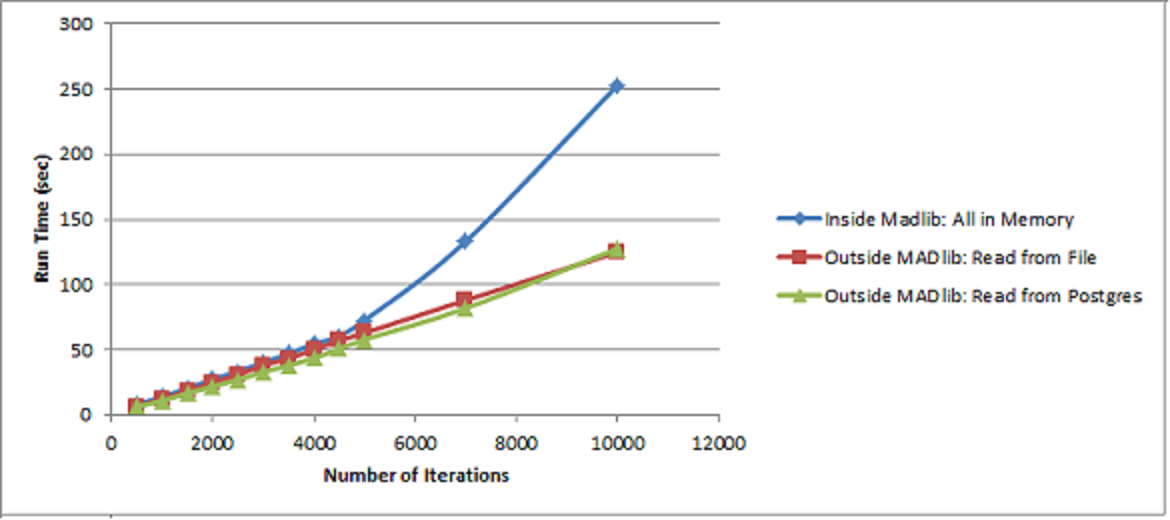
\includegraphics[height=180px]{ada1.png}
\caption{Runtimes of AdaBoost algorithm inside and outside MADlib.}
\label{fig:adainout}
\end{figure}


\begin{figure}[ht]
\centering
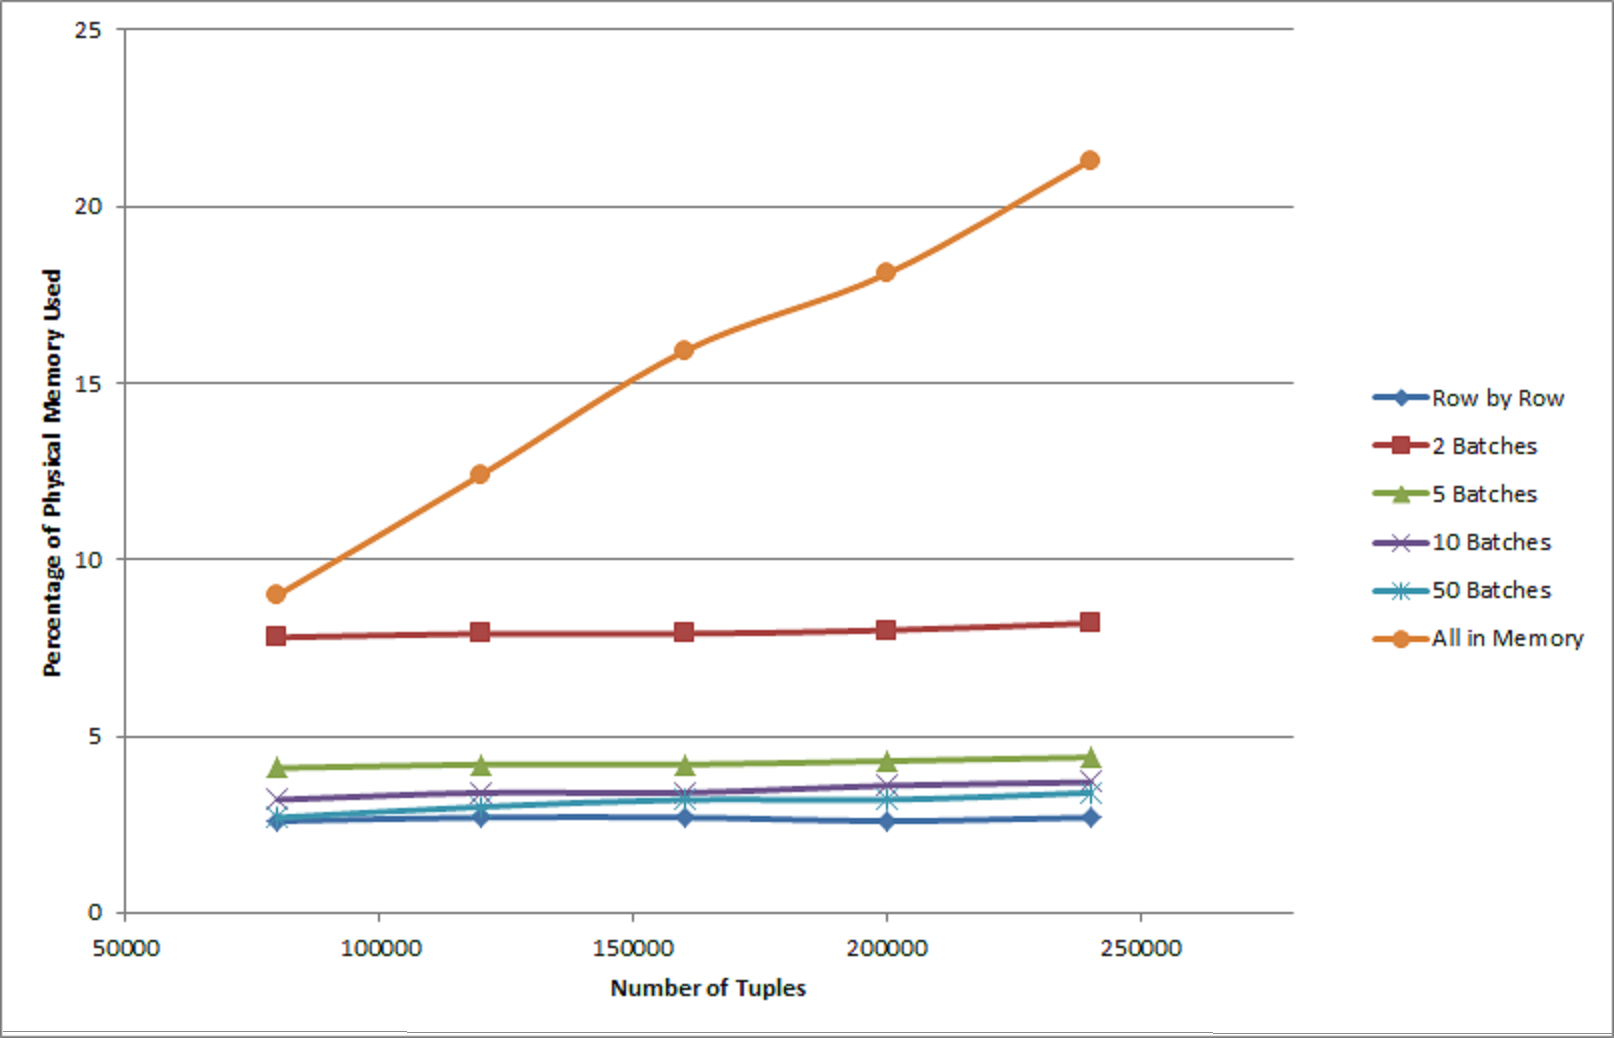
\includegraphics[height=180px]{ada4.png}
\caption{Memory usage by AdaBoost algorithm on synthetic dataset.}
\label{fig:adamem}
\end{figure}

\begin{figure}[ht]
\centering
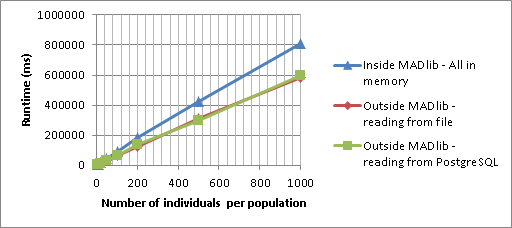
\includegraphics[height=180px]{gp-inside-vs-outside.png}
\caption{Runtimes of symbolic regression inside and outside MADlib.}
\label{fig:gp-inside-vs-outside}
\end{figure}

\subsubsection*{\itshape Performance inside and outside MADlib}
Figure \ref{fig:gp-inside-vs-outside} also compares the runtime between different execution environments: within MADlib, outside MADlib reading from a file and outside MADlib reading from the PostgreSQL database. The code used was strictly identical in older to ensure a fair comparison between execution environments. Also, all the data was loaded in memory at the beginning of the program.

~~\\
First of all, in the case of the dataset that we used to perform symbolic regression, which contains 100,000 rows and of size 2686 KB, on average reading from a file takes 230 ms whereas it takes 510 ms reading from the PostgreSQL database. TODO: Sumaiya, explain your difference.

~~\\
The most intriguing result is the runtime within MADlib, which is significantly slower than the runtime outside MADlib. This result cannot be explain by the fact that querying the database makes running within MADlib slower since running outside MADlib reading from the PostgreSQL doesn't have the issue, and the difference of runtime increases when the number of iterations increases, which means the reason isn't a fixed cost.

~~\\
To investigate this difference of runtime we bypassed MADlib and created PL/Python test case that narrows down the issue:

\begin{verbatim}
CREATE FUNCTION pymax7a (b integer)
  RETURNS float
AS $$
  import time
  start = time.time()
  a = 0
  for i in range(b):
    for ii in range(b):
      a = (((i+ii)%100)*149819874987)
  end = time.time()
  plpy.info("Time elapsed in Python: " + str((end - start)*1000) + ' ms')
  return a
$$ LANGUAGE plpythonu;
\end{verbatim}

We compared the latter code this the following identical Python code:
\begin{verbatim}
import time
import sys

def pymax7 (b):     
    a = 0
    for i in range(b):
        for ii in range(b):
            a = (((i+ii)%100)*149819874987) # keeping Python busy
    return a

def main():    
    numIterations = int(sys.argv[1])        
    start = time.time()
    print pymax7(numIterations)
    end = time.time()
    print "Time elapsed in Python:"
    print str((end - start)*1000) + ' ms'        

if __name__ == "__main__":
    main()
\end{verbatim}




\subsubsection*{\itshape Performance of batched execution.}
\begin{figure}[ht]
\centering
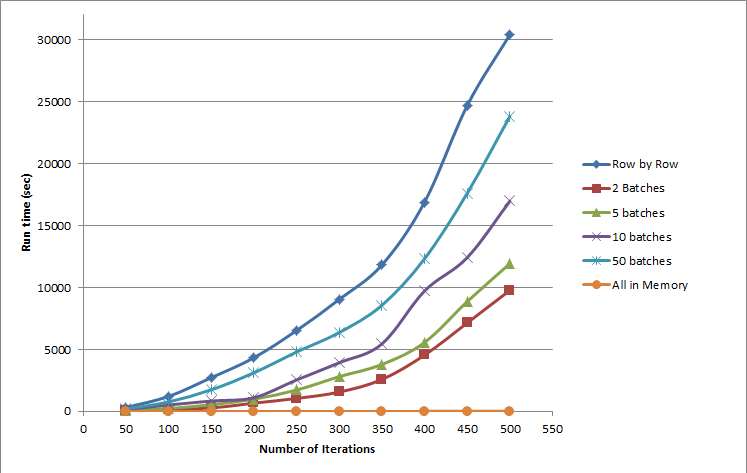
\includegraphics[height=180px]{ada2.png}
\caption{Runtimes of row-by-row, batched and all-in-memory execution of AdaBoost algorithm on BUPA liver disorder dataset.}
\label{fig:adabatch1}
\end{figure}

\begin{figure}[ht]
\centering
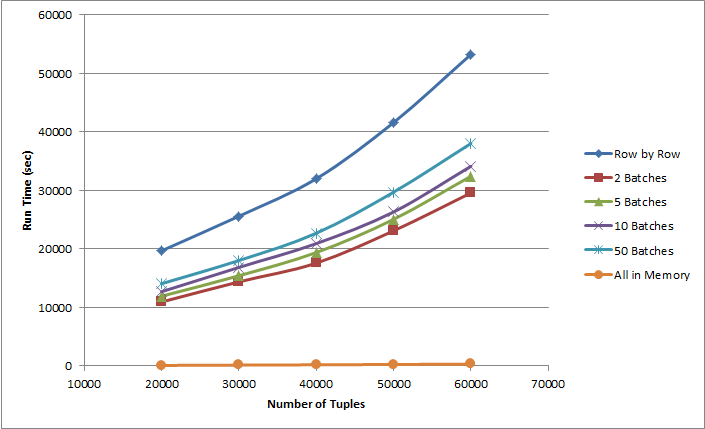
\includegraphics[height=180px]{ada3.png}
\caption{Runtimes of row-by-row, batched and all-in-memory execution of AdaBoost algorithm on synthetic dataset.}
\label{fig:adabatch2}
\end{figure}

